\chapter{Практическая часть}
\section{Задание}\label{задание}
Реализовать построение линий тока для заданного двухмерного векторного поля на четырехугольной, треугольной и гибридной сетке.
\section{Входные данные. Формат модели .msh}
Входные данные, а именно
\begin{enumerate}
	\item[---] список вершин модели;
	\item[---] список конечных элементов, описанных наборами вершин;
	\item[---] значение векторного поля в вершинах;
\end{enumerate}
загужаются в программу из исходного файла формата \verb|.msh|. Рассмотрим данный формат. Полное описание можно найти здесь \url{https://www.manpagez.com/info/gmsh/gmsh-2.4.0/gmsh_56.php}.
\subsection{Структура формата .msh}
Формат полного файла модели в формате \verb|.msh|:
\begin{verbatim}
	$MeshFormat
	version-number file-type data-size
	$EndMeshFormat
	$Nodes
	number-of-nodes
	node-number x-coord y-coord z-coord
	…
	$EndNodes
	$Elements
	number-of-elements
	elm-number elm-type number-of-tags < tag > … node-number-list
	…
	$EndElements
	$PhysicalNames
	number-of-names
	physical-dimension physical-number "physical-name"
	…
	$EndPhysicalNames
	$NodeData
	number-of-string-tags
	< "string-tag" >
	…
	number-of-real-tags
	< real-tag >
	…
	number-of-integer-tags
	< integer-tag >
	…
	node-number value …
	…
	$EndNodeData
	$ElementData
	number-of-string-tags
	< "string-tag" >
	…
	number-of-real-tags
	< real-tag >
	…
	number-of-integer-tags
	< integer-tag >
	…
	elm-number value …
	…
	$EndElementData
	$ElementNodeData
	number-of-string-tags
	< "string-tag" >
	…
	number-of-real-tags
	< real-tag >
	…
	number-of-integer-tags
	< integer-tag >
	…
	elm-number number-of-nodes-per-element value …
	…
	$ElementEndNodeData
\end{verbatim}
Рассмотрим по отдельности важные для нас части файла.
\begin{enumerate}
	\item 
	\begin{verbatim}
		$MeshFormat
		version-number file-type data-size
		$EndMeshFormat
	\end{verbatim}
	Эта секция хранит в себе информацию о версии формата, типе кодировки текста и количестве байт необходимых для хранения чисел с плавающей точкой.
	
	\item
	\begin{verbatim}
		$Nodes
		number-of-nodes
		node-number x-coord y-coord z-coord
		...
		$EndNodes
	\end{verbatim}
	Эта секция хранит в себе информацию о вершинах модели, а также общее количество вершин. Например
	\begin{verbatim}
		$Nodes
		431
		1 0 0 0
		2 0.1 0 0
		3 0.1 0.3 0
		4 0 0.3 0
		5 0.009999999999982483 0 0
		6 0.019999999999956 0 0
		...
		$EndNodes
	\end{verbatim}
	Первая строчка содержит общее количество вершин. В каждой следующей строчке записаны последовательно: номер вершины, её координаты $x,y,z$. Для двухмерных моделей всё равно записываются 3 координаты, просто $z$ оставляют равным 0.
	
	\item
	\begin{verbatim}
		$Elements
		number-of-elements
		elm-number elm-type number-of-tags <tag> … node-number-list
		…
		$EndElements
	\end{verbatim}
	В этой секции записаны конечные элементы. В первой строчке записано их общее количество. В остальных строчках записана информация о каждом из элементов:
	\begin{itemize}
		\item номер элемента
		\item тип элемента (см. раздел \ref{elem_types})
		\item количество \textit{тэгов} элемента
		\item перечислены все \textit{тэги} элемента
		\item перечислены по их номерам все вершины элемента
	\end{itemize}
	Теги элемента - разнообразная дополнительная информация об элементе. Например для улучшения визуализации в тэгах можно оставить информацию о том, каким цветом программа должна отрисовывать элемент на экран. Разработанная программа пропускает тэги элемента, поскольку они не играют важной роли при решении задачи построения линий тока.
	
	Пример данной секции файла:
	\begin{verbatim}
		$Elements
		780
		1 2 0 71 212 303
		2 2 0 105 230 281
		3 2 0 106 229 282
		...
		851 2 0 84 339 429
		852 2 0 155 397 376
		$EndElements
	\end{verbatim}
	\item 
	\begin{verbatim}
		$PhysicalNames
		...
		$EndPhysicalNames
	\end{verbatim}
	Пропускаем этот раздел. Он не несет в себе важной для решения задачи построения линий тока информации.
	\item
	\begin{verbatim}
		$NodeData
		number-of-string-tags
		< "string-tag" >
		…
		number-of-real-tags
		< real-tag >
		…
		number-of-integer-tags
		< integer-tag >
		…
		node-number value …
		…
		$EndNodeData
	\end{verbatim}
	Данная часть файла содержит дополнительную информацию (тэги) о вершинах. Именно она будет использоваться для хранения значений векторного поля в вершинах модели.
	
	Первая строчка содержит информацию о количестве тэгов -- строк, далее их перечисление.
	
	Первая строчка после тэгов -- строк содержит информацию о количестве тэгов -- действительных чисел, далее их перечисление.
	
	Первая строчка после тэгов -- действительных чисел содержит информацию о количестве тэгов -- целых чисел, далее их перечисление.
	
	Далее построчно идет информация о каждой вершине в формате: номер вершины, значения...
	
	На примере подписан смысл каждых значений тегов:
	\begin{verbatim}
		$NodeData
		1           один тег строка
		"Scalar"    тип значений "скаляры"
		1           один тег действительное число
		0           начальный момент времени 0
		3           три тега целых числа
		0           шаг времени (не используется программой)
		3           количество скаляров в каждой вершине
		16          количество вершин с доп. данным
		1 10 2.5 0
		2 10 2.5 0
		3 10 2.5 0
		...
		$EndNodeData
	\end{verbatim}
	\item
	\begin{verbatim}
		$ElementData
		…
		$EndElementData
	\end{verbatim}
	Пропускаем этот раздел. Он не несет в себе важной для решения задачи построения линий тока информации.
	\item
	\begin{verbatim}
		$ElementNodeData
		…
		$ElementEndNodeData
	\end{verbatim}
	Пропускаем этот раздел. Он не несет в себе важной для решения задачи построения линий тока информации.
\end{enumerate}
\subsection{Типы элементов в формате .msh}\label{elem_types}
При определении каждого элемента указывается его \textit{тип} -- второе число в строке информации об элементе:
\begin{Verbatim}[commandchars=+\[\]]
	1 +underline[3] 0 5 6 2 1
\end{Verbatim}
Данное число соотвествует определенному типу КЭ, список КЭ, которые планируется поддерживать программой:
\begin{itemize}
	\item Двухмерные КЭ (\textit{полностью реализованы}):
	\begin{enumerate}
		\item[2 ---] треугольник
		\item[3 ---] четырехугольник
	\end{enumerate}
	
	\item Трехмерные КЭ (\textit{планируется реализовать позже}):
	\begin{enumerate}
		\item[4 ---] тетраэдр
		\item[5 ---] гексаэдр
		\item[6 ---] прямоугольная призма с треугольным основанием
		\item[7 ---] пирамида с квадратным основанием
	\end{enumerate}
\end{itemize}
\section{Реализация на языке программирования C++}
\subsection{Ход работы алгоритма}
Программа реализовывает метод, описанный в разделе \ref{method}.
\begin{enumerate}
	\item Считать файл в формате \verb|.msh|, сформировать массив вершин, КЭ, записать координаты и значения векторного поля;
	\item Выполнить алгоритм, описанный в разделе \ref{method};
	\item Вывести полученную линию тока $L$ в формате \verb|.geo| (см. раздел \ref{geo_format} \nameref{geo_format})
\end{enumerate}

Опустим обзор реализации таких примитивов как точка (вершина), координаты, прямая, векторное поле, а также прочих вспомогательных функций и объектов, поскольку их принцип работы тривиален. Также опустим реализацию считывания данных из формата \verb|.msh| и их вывод в формате \verb|.geo|, так как она представляет собой просто считывание и печать в файлы в строгом соотвествии с форматом.

Рассмотрим подробнее основную часть алгоритма, а именно реализацию функций $I, E, A$ (см. раздел \ref{method}):
\begin{itemize}
	\item $I$ --- индикатор, проверка нахождения точки в заданном КЭ;
	\item $E$ --- определение текущего элемента по текущей точке;
	\item $A$ --- интерполяция значений векторного поля в вершинах КЭ для текущей точки.
\end{itemize}
\subsection{Определение положения точки относительно конечного элемента}
Рассмотрим методы решения задачи о принадлежности точки выпуклому многоугольнику.
\paragraph{Метод векторных произведений}
%Каноническое уравнение прямой, заданной по двум точкам $A,B$
%\begin{equation*}
%	\frac{x-x_A}{x_B-x_A} = \frac{y-y_A}{y_B-y_A}
%\end{equation*}
Направляющий вектор прямой заданной по двум точкам $A,B$
\begin{equation*}
	\vec{n} = \begin{pmatrix}
		x_B-x_A\\
		y_B-y_A
	\end{pmatrix}
\end{equation*}
Каждое ребро плоского КЭ можно описать, как часть прямой заданной по двум вершинам этого ребра. Рассмотрим точку $O$, положение которой относительно прямой можно определить с помощью векторного произведения. В зависимости от положения точки векторное произведение будет иметь положительное или отрицательное направление по оси $z$, см. Рисунок \ref{vec_example} (a) и (b) соответственно.
\begin{figure}[H]
	\hfill
	\begin{subfigure}{.45\textwidth}
		\centering
		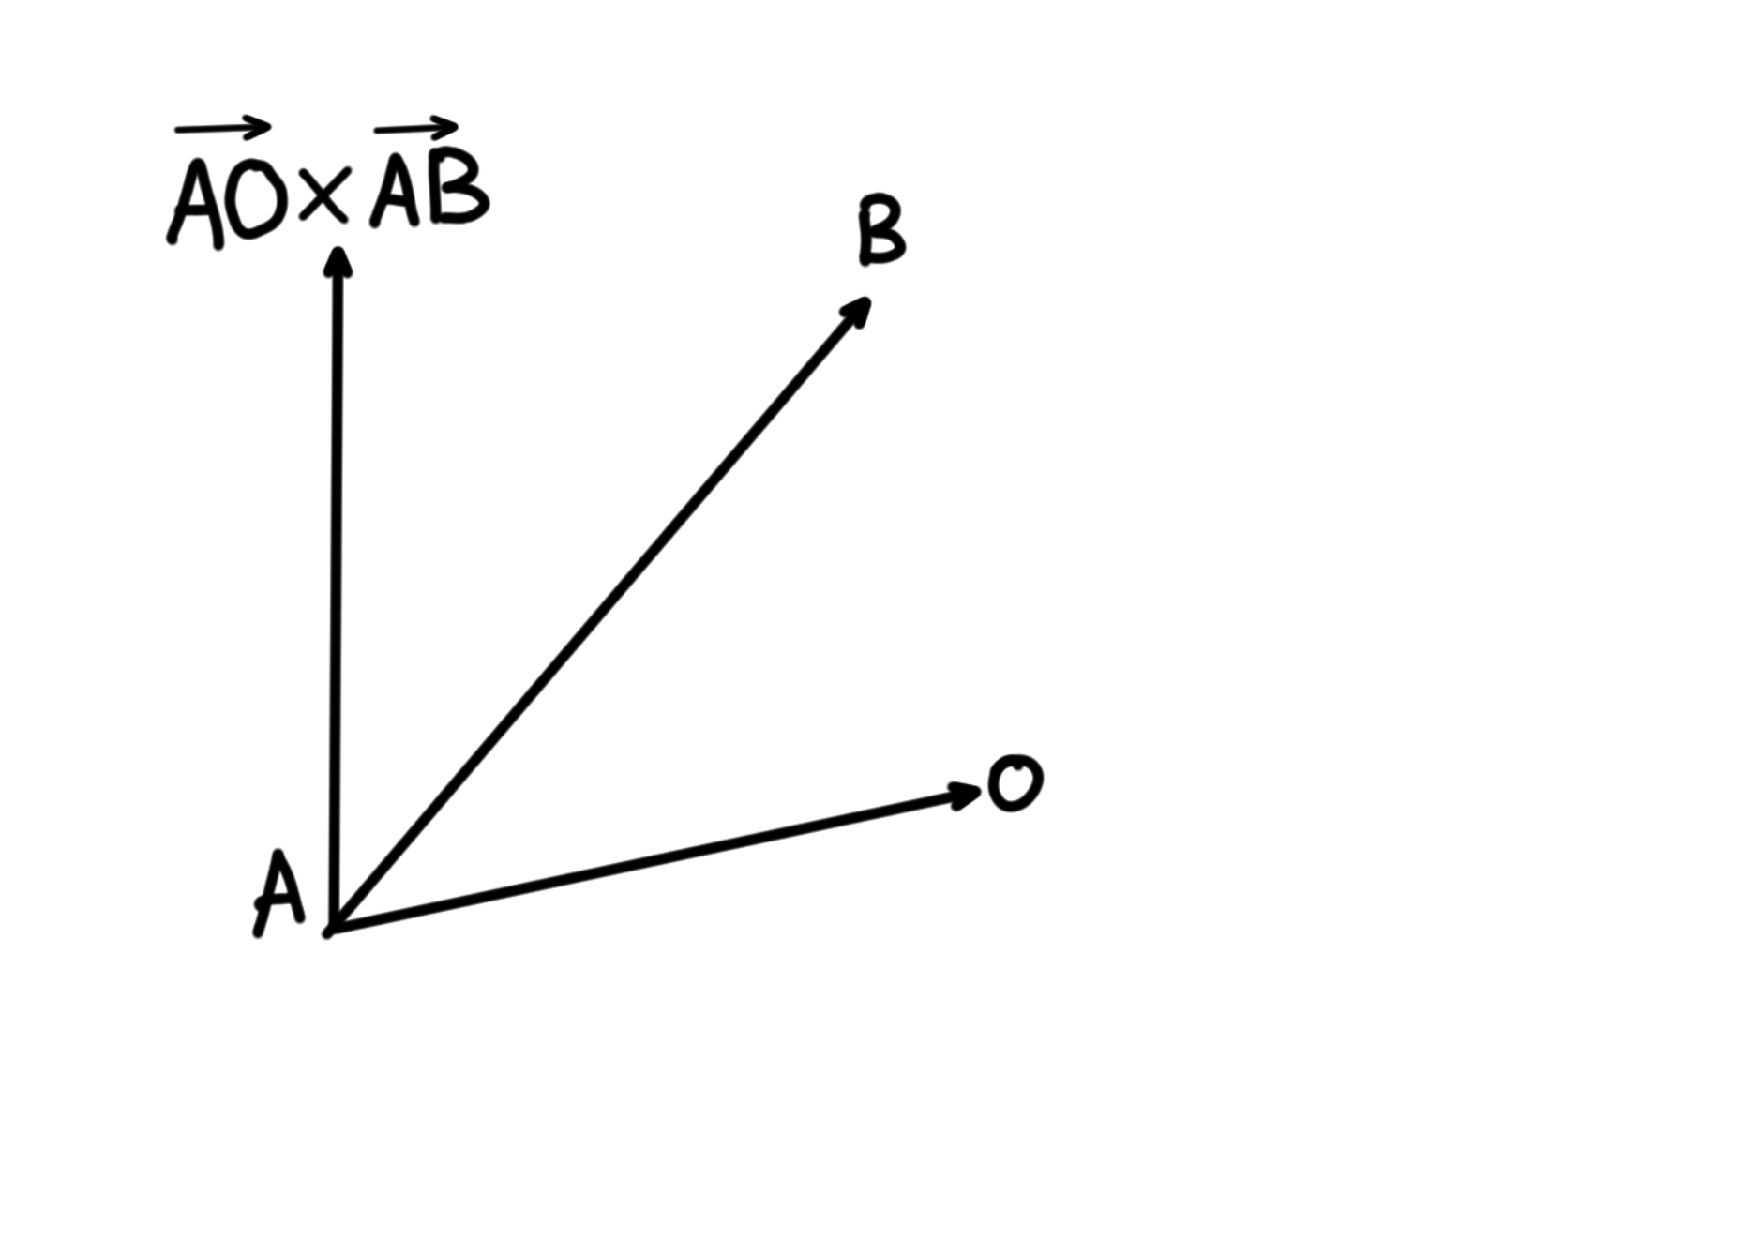
\includegraphics[width=\linewidth,page=1,trim={2cm 5cm 11cm 2cm}]{img/gm}
		\caption{Точка справа от прямой, векторное произведение положительное}
	\end{subfigure}
	\hfill
	\begin{subfigure}{.45\textwidth}
		\centering
		\includegraphics[width=\linewidth,page=2,trim={2cm 0cm 8cm 1cm}]{img/gm}
		\caption{Точка слева от прямой, векторное произведение отрицательное}
	\end{subfigure}
	\hfill
	\caption{Применение векторного произведения для определения положения точки относительно прямой}
	\label{vec_example}
\end{figure}

Просчитав векторное произведение направляющего вектора $\vec{n}$ каждого ребра многоугольника с вектором из первой его вершины в точку $O$, положение которой необходимо определить, можно сделать вывод, о положении точки относительно выпуклого многоугольника. Если точка внутри, то все векторные произведение будут направлены в положительном направлении, иначе точка находится вне многоугольника (см. примеры с параллелепипедом (a) и треугольником (b) на Рисунке \ref{vec_method}).
\begin{figure}[H]
	\hfill
	\begin{subfigure}{.55\textwidth}
		\centering
		\includegraphics[width=\linewidth,page=3,trim={0cm 7cm 3cm 0cm}]{img/gm}
		\caption{Точка внутри параллелепипеда, все векторные произведение направлены в положительном направлении}
	\end{subfigure}
	\hfill
	\begin{subfigure}{.35\textwidth}
		\centering
		\includegraphics[width=\linewidth,page=4,trim={4cm 7cm 12cm 0cm}]{img/gm}
		\caption{Точка вне треугольника, одно из векторных произведений направлено в отрицательном направлении}
	\end{subfigure}
	\hfill
	\caption{Применение векторного произведения для решения задачи принадлежности точки многоугольнику}
	\label{vec_method}
\end{figure}

Таким образом можно определить находится ли точка внутри выпуклого многогранника. Этот метод удобен, так как не ограничивает тип сетки, а в качестве КЭ примет любой n-угольник.
Направляющий вектор прямой имеет вид:
\begin{equation*}
	\vec{AB} = \vec n = \begin{pmatrix}
		x_B - x_A\\
		y_B - y_A\\
		0
	\end{pmatrix}.
\end{equation*}
Вектор $AO$ задаётся аналогично:
\begin{equation*}
	\vec {AO} = \begin{pmatrix}
		x_O - x_A\\
		y_O - y_A\\
		0
	\end{pmatrix}
\end{equation*}
Тогда векторное произведение $\vec{AO}\times\vec{AB}$ легко посчитать следующим образом:
\begin{multline*}
	\vec{AO}\times\vec{AB} = \left|\begin{array}{ccc}
		\vec{x} & \vec{y} & \vec{z} \\
		x_B - x_A & y_B - y_A & 0 \\
		x_O - x_A & y_O - y_A & 0 \\
	\end{array}\right| =\\= \vec{z}\cdot\left(\left(x_B - x_A\right)\cdot\left(y_O - y_A\right) - \left(y_B - y_A\right)\cdot\left(x_O - x_A\right)\right)
\end{multline*}
Следовательно выражение $\left(x_B - x_A\right)\cdot\left(y_O - y_A\right) - \left(y_B - y_A\right)\cdot\left(x_O - x_A\right)$ в зависимости от его знака будет определять положение точки. Код программы для определения положения точки относительно прямой:
\lstinputlisting[language=C++, firstline=16, lastline=27]{current-lines/src/Geometry/Line.cpp}

Код программы для определения положения точки относительно конечного элемента:
\lstinputlisting[language=C++, firstline=147, lastline=155]{current-lines/src/Element/Element.cpp}
Здесь программа циклично проверяет положение точки относительно каждого ребра. Также дополнительно добавлена проверка того, что точка находится в диапазоне значений $x$ и $y$ для данного элемента. Эта проверка позволяет сразу сказать, что точка лежит вне КЭ, если она находится очень далеко от него.
\paragraph{Метод трассировки лучей}
Рассмотрим выпуклый многоугольник. Необходимо определить, находится ли заданная точка внутри него. Алгоритм можно описать следующим образом:
\begin{enumerate}
	\item Из тестируемой точки выпускается луч либо в заранее заданном, либо в произвольном направлении;
	\item Считается количество пересечений с многоугольником;
	\item Если количество пересечений четное, точка находимся снаружи. Если количество пересечений нечетное, точка – внутри (см. Рисунок \ref{trace_method});
\end{enumerate}
\begin{figure}[H]
	\centering
	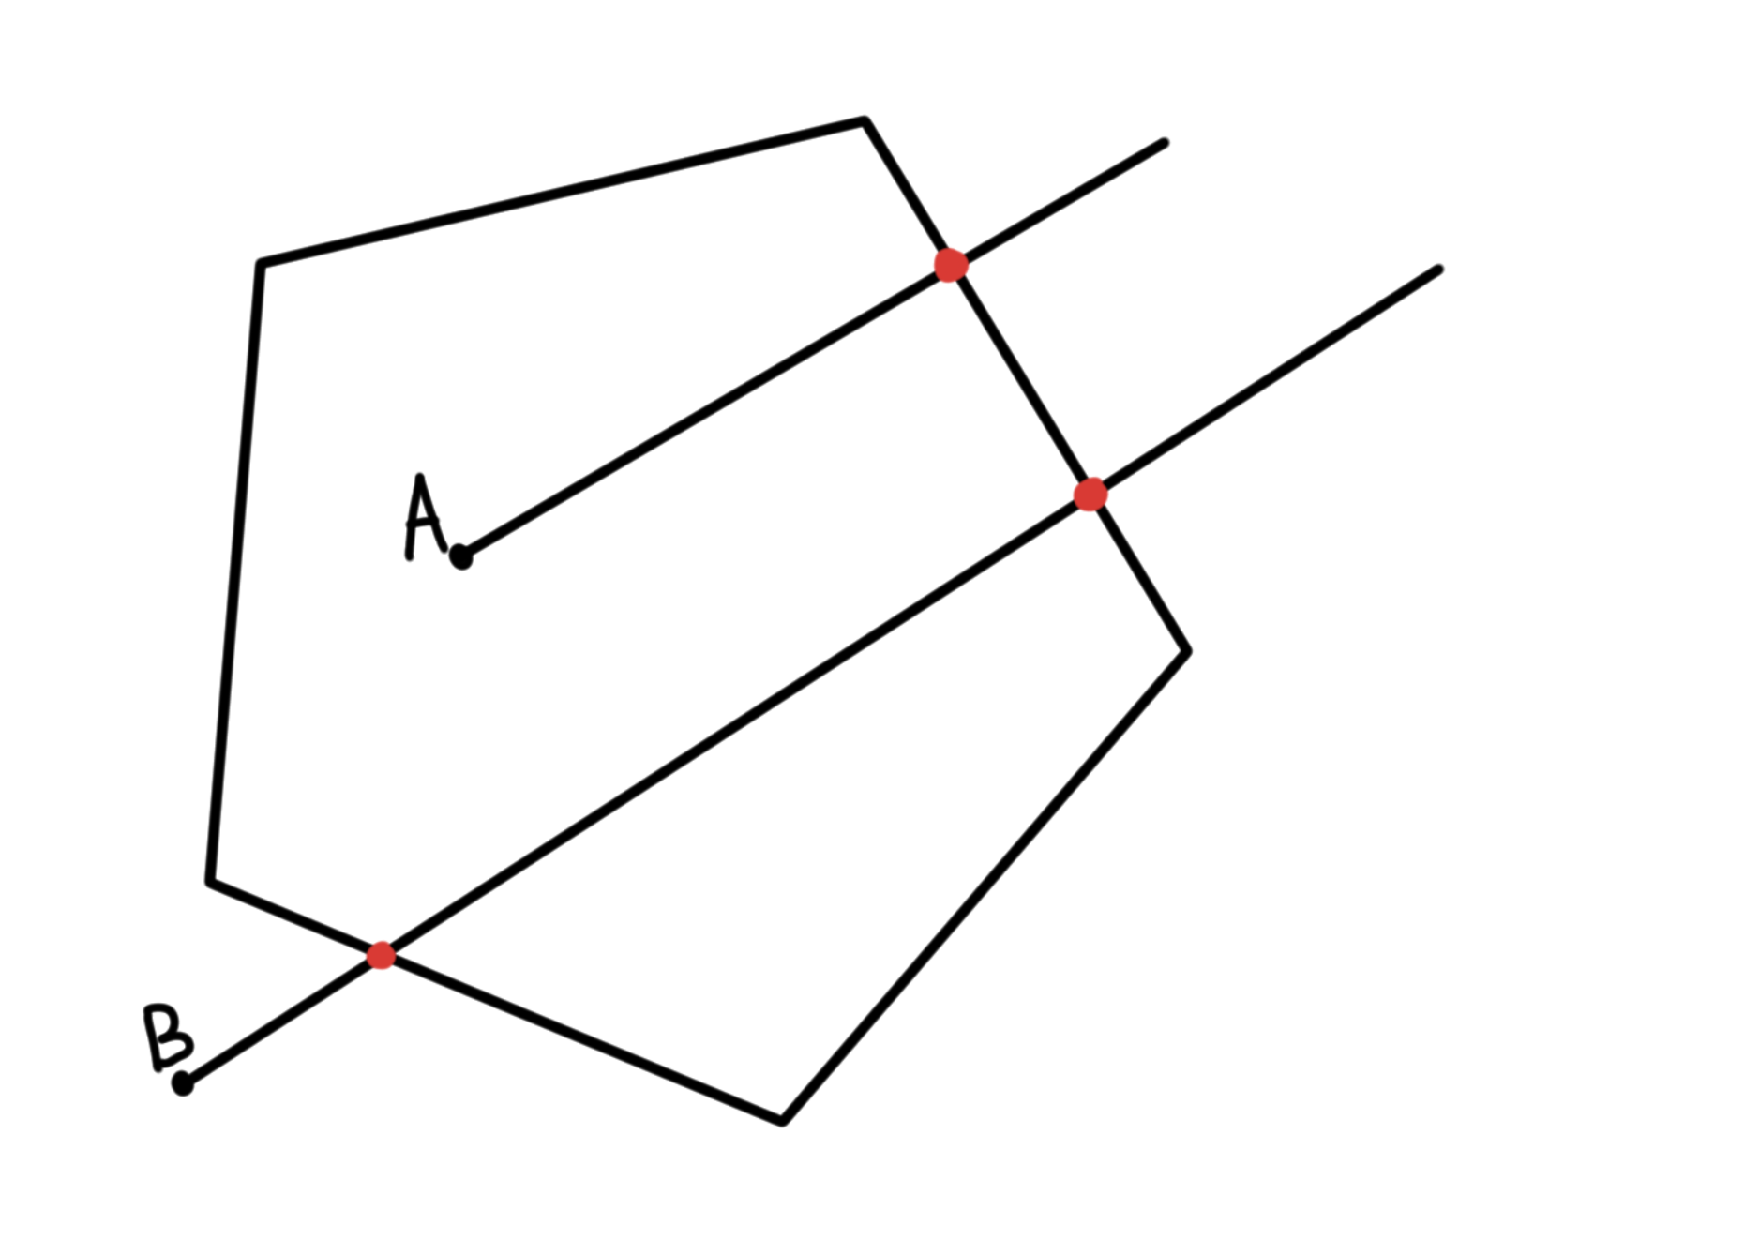
\includegraphics[width=.6\linewidth,trim={2cm 2cm 5cm 2cm}]{img/gmtrace}
	\caption{Применение трассировки для решения задачи принадлежности точки многоугольнику. Для точки $A$ найдено одно пересечение (следовательно, она внутри), для точки $B$ найдено два пересечения (следовательно, она снаружи)}
	\label{trace_method}
\end{figure}
\lstinputlisting[language=C++, firstline=159, lastline=172]{current-lines/src/Element/Element.cpp}
Полное описание метода см. \cite{pnpoly}.
%\subsection{Нумерация узлов КЭ}
Для корректной работы метода векторных произведений для определения положения точки относительно КЭ требуется, чтобы узлы КЭ были перечислены в порядке по часовой стрелке. При разработке алгоритма было принято определение ребра, как двух подряд идущих вершин. Если вершины будут пронумерованы не по порядку, то при обработке ребра алгоритм на самом деле будет обрабатывать отрезок, лежащий внутри КЭ, а не ребро.

Формат \verb|.msh| не гарантирует, что ребра пронумерованы в соответствие с определением ребра выше. 

Необходимо реализовать специальный алгоритм сортировки вершин КЭ по часовой стрелке. Ключевая вещь, необходимая алгоритму сортировки -- это возможность сравнить два элемента массива. Следовательно нужно создать функцию, которая будет сравнивать две точки и расставлять их по порядку по часовой стрелке.

\subsubsection{Сравнение двух точек}
\lstinputlisting[language=C++, firstline=21, lastline=52]{current-lines/src/Element/Element.cpp}
Точки сортируются относительно угла $\frac{\pi}{2}$ по часовой стрелке. Началом координат будеv считать предварительно заданную точку $C$ -- центр. 

\paragraph{Простые случаи}
Сперва сравним координаты $x$ точек, если они находятся в разных полуплоскостях относительно центра, то можно сразу сделать вывод о том, какая из них больше.

Если точки находятся на вертикальной прямой $x=C_x$, то сравним их по удаленности от центра $|y-C_y|$.

\paragraph{Общий случай}
Посчитаем векторное произведение $\vec{CA}\times\vec{CB}$ и в зависимости от его знака определим относительное положение точек $A$ и $B$ (аналогично тому, как это было сделано при определении принадлежности точки многограннику).

\paragraph{Точки с одинаковым значением угла}
Для точек с одинаковым значением угла векторное произведение $\vec{CA}\times\vec{CB}$ будет равным $\vec{0}$, тогда сравним их по удалённости от центра $|CA|, |CB|$.

\paragraph{О производительности}
Для сравнения точек можно было применить также функцию $\operatorname{atan2}$, определяемую следующим образом
\begin{equation*}
	\operatorname{atan2}(y,x)=\begin{cases}
			\arctan(\frac{y}{x}), &x>0,\\
			\arctan(\frac{y}{x})+\pi, &x<0 \wedge y\geq 0,\\
			\arctan(\frac{y}{x})-\pi, &x<0 \wedge y<0,\\
			+\frac{\pi}{2}, &x=0 \wedge y>0,\\
			-\frac{\pi}{2}, &x=0 \wedge y<0,\\
			\varnothing, &x=0\wedge y=0.
		\end{cases}
\end{equation*}
Одним лишь сравнением значений $\operatorname{atan2}$ для точек $A$ и $B$ можно их упорядочить. Но данная функция затрачивает намного больше вычислительных возможностей компьютера, поскольку использует деление чисел с плавающей точкой и вычисление тригонометрических функций. Предложенное ранее сравнение двух точек использует только операции сложения(вычитания) и умножения, что делает её намного производительнее.

\subsubsection{Сортировка}
Испольуется алгоритм сортировки \verb|std::sort| из стандартной библиотеки \verb|C++|, центр сортировки вычисляется предварительно как среднее арифметическое координат всех вершин КЭ.
\lstinputlisting[language=C++, firstline=65, lastline=75]{current-lines/src/Element/Element.cpp}


\subsection{Интерполяция в КЭ}
\subsubsection{Интерполяция на четырехугольном КЭ}
\paragraph{Билинейная интерполяция}
Пусть в четырёх узлах КЭ (обозначены красным) $Q_{11}, Q_{12}, Q_{21}, Q_{22}$ с координатами $x_1, y_1; x_2, y_2; x_3, y_3; x_4, y_4;$ значения исходной функции известны. Требуется получить приближённое (интерполированное) значение исходной функции в точке $P$ (обозначена зеленым) с координатами $x, y$ (см. Рисунок \ref{Bilinear_interpolation}).
\begin{figure}[H]
	\centering
	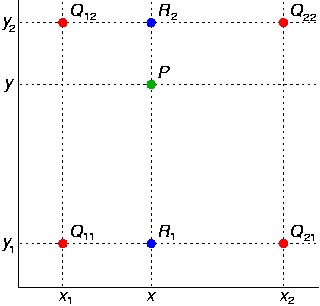
\includegraphics[width=0.4\linewidth]{img/Bilinear_interpolation}
	\caption{Постановка задачи билинейной интерполяции}
	\label{Bilinear_interpolation}
\end{figure}
Первым шагом линейно интерполируется значение вспомогательных синих точек $R_1, R_2$ (обозначены синим) вдоль оси абсцисс, где
\begin{equation*}
	R_1 = (x,y_1),\quad R_2 = (x,y_2),
\end{equation*}
тогда
\begin{equation*}
	\begin{array}{cc}
		f(R_1)\approx \tau f(Q_{11}) + (1-\tau)f(Q_{21})\\
		f(R_2)\approx \tau f(Q_{112}) + (1-\tau)f(Q_{22})
	\end{array}\quad
	\tau = \frac{x_2-x}{x_2-x_1}
\end{equation*}

При вычислении $\tau$ по данной формуле в четырехугольном КЭ отличном от прямоугольника, может получиться $\tau>1$. Чтобы учесть этот случай, будем ограничивать $\tau$ следующим образом
\begin{equation*}
	\tau = \min\left\{1,\, \frac{x_2-x}{x_2-x_1}\right\}.
\end{equation*}

Теперь проводится линейная интерполяция между вспомогательными точками $R_1, R_2$. В результате получаем:
\begin{equation*}
	f(P)\approx pf(R_1) + (1-p)f(R_2)\quad p=\frac{y_2-y}{y_2-y_1}
\end{equation*}
Это и есть интерполируемое значение функции $f(x,y)$, причём значения интерполирующей функции $F(x,y)$ равны значениям интерполируемой функции в исходных точках $Q_{11}, Q_{12}, Q_{21}, Q_{22}$.
\begin{align*}
	f(x,y) \approx F(x, y) = & \frac{f(Q_{11})}{(x_2-x_1)(y_2-y_1)} (x_2-x)(y_2-y)\ + \\
	+                        & \frac{f(Q_{21})}{(x_2-x_1)(y_2-y_1)} (x-x_1)(y_2-y)\ + \\
	+                        & \frac{f(Q_{12})}{(x_2-x_1)(y_2-y_1)} (x_2-x)(y-y_1)\ + \\
	+                        & \frac{f(Q_{22})}{(x_2-x_1)(y_2-y_1)} (x-x_1)(y-y_1).
\end{align*}
Код программы для метода билинейной интерполяции:
\lstinputlisting[language=C++, firstline=7, lastline=36]{current-lines/src/Element/QuadrangleElement.cpp}
\subsubsection{Интерполяция на треугольном КЭ}
\paragraph{Наивный метод}
Рассмотрим треугольник на Рисунке \ref{trig}.
\begin{figure}[H]
	\centering
	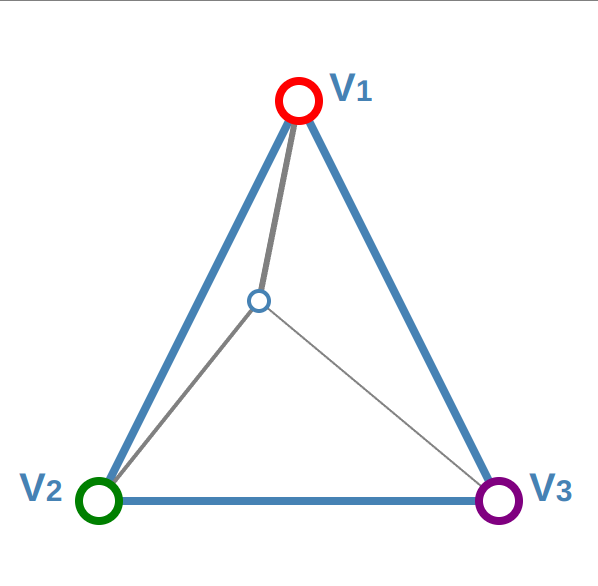
\includegraphics[width=0.4\linewidth,trim={0 0 0 1cm},clip]{img/trig}
	\caption{Треугольник для интерполяции}
	\label{trig}
\end{figure}
Расстояния от точки $P$ до вершин
\begin{align*}
	|P V_1| &= \sqrt{(X_{v1} - P_{x})^2 + (Y_{v1} - P_{y})^2}\\
	|P V_2| &= \sqrt{(X_{v2} - P_{x})^2 + (Y_{v2} - P_{y})^2}\\
	|P V_3| &= \sqrt{(X_{v3} - P_{x})^2 + (Y_{v3} - P_{y})^2}
\end{align*}
Расстояния принимают большие значения, когда точка находимся далеко, и маленькие - когда точка находимся близко. Поэтому инвертируем их, чтобы большие значения придавали больший вес более близким вершинам. Другими словами, мы будем интерполировать обратно пропорционально расстоянию до каждой вершины. \cite{trig_interpolate}
\begin{align*}
	W_{v1} &= 1 - \frac{|P V_1|}{|P V_1|+|P V_2|+|P V_3|}\\
	W_{v2} &= 1 - \frac{|P V_2|}{|P V_1|+|P V_2|+|P V_3|}\\
	W_{v3} &= 1 - \frac{|P V_3|}{|P V_1|+|P V_2|+|P V_3|}
\end{align*}
Это решение простое, его легко начать использовать и оно достаточно интуитивно понятно. Но оно даёт не очень хорошие результаты, если треугольник для интерполяции оказывается вытянутым (см. Рисунок \ref{tri-int-naive-slant}). 
\begin{figure}[H]
	\centering
	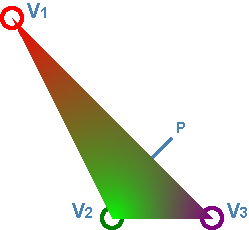
\includegraphics[width=0.45\linewidth]{img/tri-int-naive-slant}
	\caption{Интерполяция значений в треугольном КЭ с помощью наивного метода}
	\label{tri-int-naive-slant}
\end{figure}
На Рисунке \ref{tri-int-naive-slant} видно, что точка $P$, которая находится на ребре $V_1 V_3$ будет иметь значение ближе к значению в вершине $V_2$, что является не совсем правильным поведением алгоритма. В такой точке $P$ хотелось бы получить смесь значений из точек $V_1$ и $V_3$ без $V_2$. 
Код программы для наивного метода:
\lstinputlisting[language=C++, firstline=6, lastline=30]{current-lines/src/Element/GenericElement.cpp}
Перейдём к другому методу интерполяции в треугольном КЭ.

\paragraph{Метод на основе барицентрических координат}
Суть метода барицентрических координат в нахождении барицентрических координат точки $W_{v1}, W_{v2}, W_{v3}$ на основе заданных вершин $V_1, V_2, V_3$, удовлетворяющих системе уравнений \eqref{bary_cases}. \cite{trig_interpolate}
\begin{equation}\label{bary_cases}
	\begin{cases}
		P_x = W_{v1}X_{v1} + W_{v2}X_{v2} + W_{v3}X_{v3},\\
		P_y = W_{v1}Y_{v1} + W_{v2}Y_{v2} + W_{v3}Y_{v3},\\
		W_{v1} + W_{v2} + W_{v3} = 1.
	\end{cases}
\end{equation}

Решение системы \eqref{bary_cases} имеет вид:
\begin{equation*}
	\begin{cases}
		W_{v1}=\dfrac{(Y_{v2}-Y_{v3})(P_{x}-X_{v3})+(X_{v3}-X_{v2})(P_{y}-Y_{v3})}{(Y_{v2}-Y_{v3})(X_{v1}-X_{v3})+(X_{v3}-X_{v2})(Y_{v1}-Y_{v3})},\\[15pt]
		W_{v2}=\dfrac{(Y_{v3}-Y_{v1})(P_{x}-X_{v3})+(X_{v1}-X_{v3})(P_{y}-Y_{v3})}{(Y_{v2}-Y_{v3})(X_{v1}-X_{v3})+(X_{v3}-X_{v2})(Y_{v1}-Y_{v3})},\\[15pt]
		W_{v3}=1 - W_{v1} - W_{v2}.
	\end{cases}
\end{equation*}

Результаты можно увидеть на Рисунке \ref{bary_results}. Видно (см. Рисунок \ref{bary_example}), что теперь при получении значений в точках на ребрах не участвуют значения противолежащих вершин.
\begin{figure}[H]
	\hfill
	\begin{subfigure}{0.48\textwidth}
		\centering
		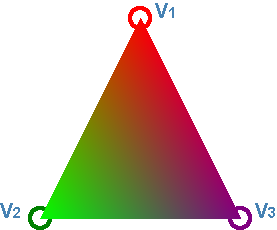
\includegraphics[width=\linewidth]{img/tri-int-bary}
		\caption{Интерполяция значений в треугольном КЭ с помощью метода на основе барицентрических координат}
		\label{tri-int-bary}
	\end{subfigure}
	\hfill
	\begin{subfigure}{0.45\textwidth}
		\centering
		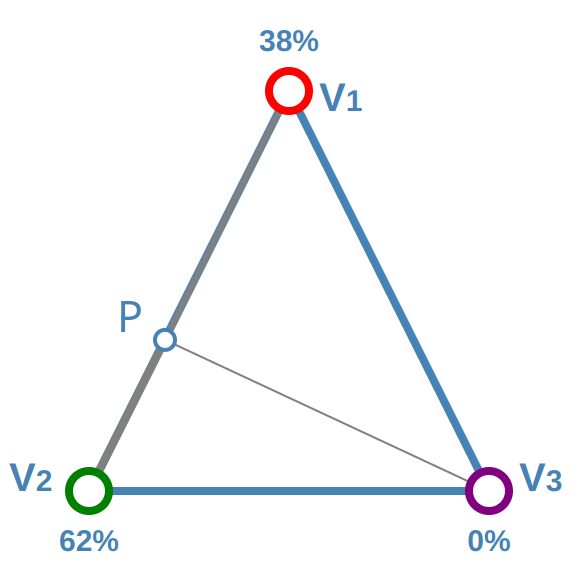
\includegraphics[width=\linewidth]{img/bary_example}
		\caption{Пример интерполяции методом на основе барицентрических координат для точки, лежащей на ребре треугольника}
		\label{bary_example}
	\end{subfigure}
	\hfill
	\caption{Результаты применения метода барицентрических координат}
	\label{bary_results}
\end{figure}
Таким образом метод барицентрических координат работает более точно.

\subsection{Результаты генерации линий тока на разных типах сеток}
В процессе создания программы были реализованы следующие алгоритмы:
\begin{itemize}
	\item[---] Определение положения точки относительно КЭ:
	\begin{enumerate}[label=\arabic*)]
		\item метод на основе вычисления векторных произведений (для любых двумерных сеток),
		\item метод трассировки лучей (для любых двумерных сеток).
	\end{enumerate}
	\item[---] Сортировка вершин КЭ:
	\begin{enumerate}[label=\arabic*)]
		\item метод \verb|atan2| (не используется ввиду неэффективности),
		\item метод на основе вычисления векторных произведений.
	\end{enumerate}
	\item[---] Интерполяция значений в КЭ:
	\begin{enumerate}[label=\arabic*)]
		\item билинейная интерполяция (для четырехугольных КЭ),
		\item наивная интерполяция на основе вычисления расстояния до вершин (для любых КЭ),
		\item метод на основе барицентрических координат (для треугольных КЭ).
	\end{enumerate}
\end{itemize}

\section{Выходные данные. Формат .geo}\label{geo_format}
Для визуализации линий тока была выбрана программа \verb|gmsh|. Она позволяет интерактивно работать с моделями, сетками и другими видами геометрии, заданными в различных форматах. Удобным способом задания линий тока, который поддерживается программой \verb|gmsh|, является формат \verb|.geo|. Это очень обширный формат, позволяющий описывать сложную геометрию, полностью рассматривать его не будем. Опишем только способ задания линий тока в данном формате:
\begin{verbatim}
	Point(1) = {0.1, 0.05, 0, 1.2};
	Point(2) = {0.111707, 0.0526363, 0, 1.2};
	Point(3) = {0.123414, 0.0552719, 0, 1.2};
	Point(4) = {0.135121, 0.0579057, 0, 1.2};
	...
	Point(97) = {1.17998, 0.397062, 0, 1.2};
	Point(98) = {1.19178, 0.399233, 0, 1.2};
	Line(98) = {1, 2, 3, 4, ..., 97, 98};
\end{verbatim}
Построчно выводятся полученные точки с их номерами и тегами (необходимы для правильной визуализации) в следующем формате:
\begin{verbatim}
	Point(<номер точки>) = {<x>, <y>, <z>, <тег>};
\end{verbatim}
После задания точек выводится строка (или строки) с информацией о линии (линиях), построенных на данных точках. Строка, описывающая линию, имее следующий формат:
\begin{verbatim}
	Line(<количество точек>) = {<список номеров точек>};
\end{verbatim}

В итоге результаты работы можно увидеть выполнив команду:
\begin{verbatim}
	gmsh model.msh result.geo
\end{verbatim}
Тогда программа визуализации \verb|gmsh| отобразит исходную конечно-элементную сетку, векторное поле, заданное в её узлах, а также полученную линию тока.

Полный код программы доступен по ссылке \url{https://github.com/Plasmaa0/current-lines}.